\documentclass[11pt,a4paper]{article}

% Encoding & Sprache
\usepackage[T1]{fontenc}
\usepackage[utf8]{inputenc}
\usepackage[ngerman]{babel}

% Layout & Typografie
\usepackage[a4paper,margin=2cm]{geometry}
\usepackage{setspace}
\usepackage{enumitem}
\usepackage{hyperref}
\usepackage{graphicx}
\usepackage{array}
\usepackage{booktabs}
\usepackage{multicol}
\usepackage{longtable}
\usepackage{tabularx}
\usepackage{fancyhdr}
\usepackage{titlesec}
\usepackage{xcolor}

\hypersetup{
  colorlinks=true,
  linkcolor=black,
  urlcolor=blue,
  citecolor=black
}

% Header / Footer
\pagestyle{fancy}
\fancyhf{}
\lhead{Studiengang: HCD}
\chead{HopIn Usability Test (A6B)}
\rhead{Assignment: A6B}
\lfoot{Kevin Forter \& Benjamin Feichtlbauer \& Rohit Birdi \& Muhammad Suhail Edipoglu}
\rfoot{\thepage}

% Absätze & Listen
\setlength{\parskip}{6pt}
\setlength{\parindent}{0pt}
\setlist[itemize]{leftmargin=1.2em}
\setlist[enumerate]{leftmargin=1.4em}

% Makros
\newcommand{\appname}{\textbf{HopIn}}
\newcommand{\minisection}[1]{\vspace{0.4em}\textbf{#1}\quad}
\newcommand{\ratingscale}{
  \begin{tabularx}{0.6\linewidth}{*{7}{>{\centering\arraybackslash}p{0.9cm}}}
  \toprule
  \textbf{1} & \textbf{2} & \textbf{3} & \textbf{4} & \textbf{5} & \textbf{6} & \textbf{7}\\
  \bottomrule
  \end{tabularx}
}
\newcommand{\ratingitem}[1]{#1\\[0.3em]\ratingscale\par\vspace{0.8em}}

\begin{document}

% Titelseite
\begin{titlepage}
  \centering
  {\Large Human-Centered Design (HCD)}\\[2ex]
  {\large Assignment A6B}\\[10ex]
  {\huge \textbf{HopIn}: Moderierter Usability-Test}\\[3ex]
  {\large Testplan, Aufgaben und Messkonzept}\\[8ex]

  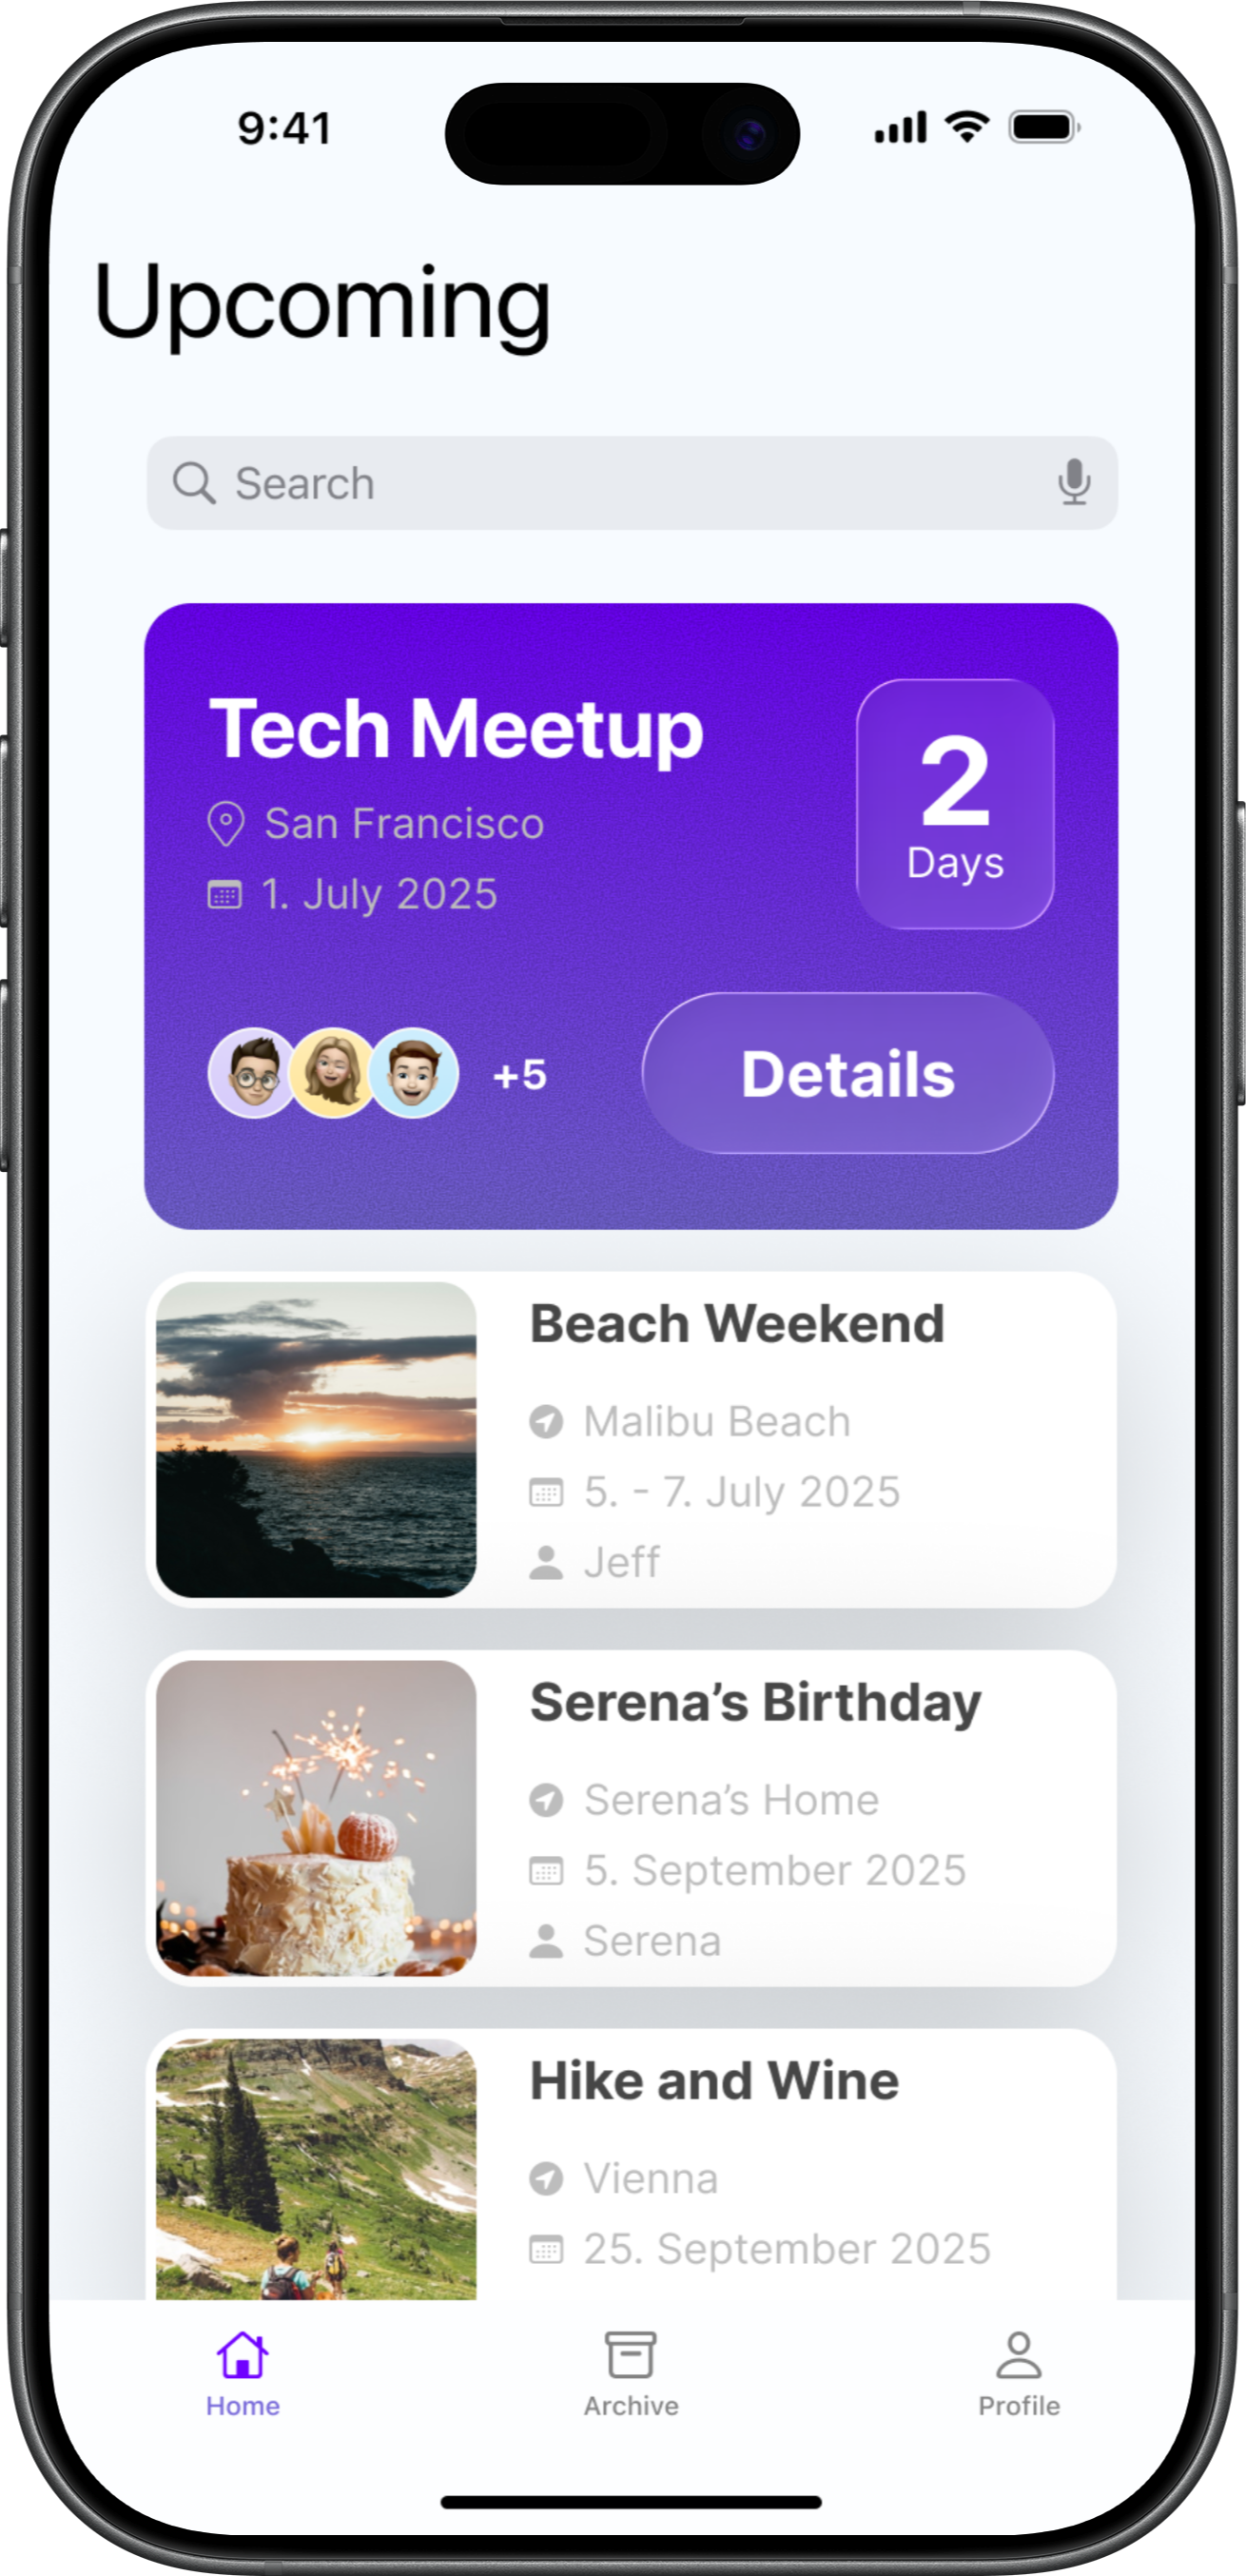
\includegraphics[width=0.4\textwidth]{images/iphone_mockup.png}\\[8ex]

  \begin{tabular}{@{}p{4cm}p{9cm}@{}}
    \textbf{Studiengang:} & HCD \\
    \textbf{Kurs / Studierende:} & Kevin Forter \& Benjamin Feichtlbauer \& Rohit Birdi \& Muhammad Suhail Edipoglu \\
  \end{tabular}

  \vfill
\end{titlepage}

\tableofcontents
\newpage

% ----------------------------------------------------------------------

\section{Beschreibung des getesteten Prototyps}
\appname{} ist eine mobile App / Web-App zur \textbf{temporären Event-Organisation} über \textbf{Gruppen}, die nach dem Anlass \textbf{automatisch archiviert} werden. Nutzerinnen und Nutzer können spontane oder kurzfristige Aktivitäten (z.\,B. Partys, Ausflüge, Sport, Uni-Projekte) gemeinsam planen, kommunizieren und durchführen. Im Unterschied zu dauerhaften Messenger-Gruppen bleibt der Kommunikationsbereich in \appname{} aufgeräumt: Nach Ende des Events verschwindet die Gruppe aus der aktiven Liste und ist im Archiv weiterhin einsehbar.

\minisection{Zentrale Funktionen (aus dem Prototyp):}
\begin{itemize}
  \item \textbf{Event-Gruppe erstellen} (Titel, Datum/Zeit, Ort, Beschreibung).
  \item \textbf{Teilnehmende einladen} (Beitrittslink / QR teilen).
  \item \textbf{Chat \& Organisation} an einem Ort: \textbf{To-Dos}, \textbf{Umfragen/Abstimmungen}, Hinweise.
  \item \textbf{Gruppe abschließen/archivieren} nach Event-Ende (automatisch).
\end{itemize}

% ----------------------------------------------------------------------

\section{Testziele gemäss Jakob Nielsen}
Wir orientieren uns an \textbf{Nielsens fünf Qualitätskomponenten} (Usability-Ziele):

\begin{enumerate}
  \item \textbf{Learnability} – Wie leicht können Erstnutzende die Hauptaufgaben durchführen?
  \item \textbf{Efficiency} – Wie schnell und reibungslos laufen die Kernflows ab?
  \item \textbf{Memorability} – Finden Nutzende nach kurzer Ablenkung schnell wieder hinein?
  \item \textbf{Errors} – Welche Fehler treten auf? Wie schwer sind sie?
  \item \textbf{Satisfaction} – Wie zufrieden sind die Nutzenden subjektiv?
\end{enumerate}

% ----------------------------------------------------------------------

\section{Rahmenbedingungen des Tests}
\begin{itemize}
  \item \textbf{Setting:} Moderierter Lab-Test (im Unterricht).
  \item \textbf{Dauer pro Person:} ca. 20 Minuten.
  \item \textbf{Rollen:} Moderator/in, Protokollant/in.
  \item \textbf{Protokoll:} Think-Aloud, neutrale Nachfragen.
  \item \textbf{Aufzeichnung:} falls möglich Bildschirmaufnahme (intern).
\end{itemize}

% ----------------------------------------------------------------------

\section{Aufgaben (Tasks)}
Die Aufgaben sind realistisch, zielbasiert und ergebnisoffen formuliert.

\subsection*{T1 – Event-Gruppe anlegen}
Sunrise-Workout Gruppe erstellen, Titel/Ort/Zeit + kurze Notiz.

\subsection*{T2 – Teilnehmende einladen}
Beitrittslink oder QR-Code finden und teilen.

\subsection*{T3 – Chat lesen}
In „Serena's Birthday“ den aktuellen Stand nachlesen.

\subsection*{T4 – To-Do hinzufügen und abhaken}
In „Boys Trip“ ein ToDo übernehmen und abhaken.

\subsection*{T5 – Archiviertes Event finden}
Das Event „Elternabend“ im Archiv öffnen.

% ----------------------------------------------------------------------

\section{Messkonzept: Was wird beobachtet / festgehalten}

Das Messkonzept dient als Orientierung für Moderator/in und Protokollant/in,
bleibt aber \textbf{bewusst flexibel}. Es beschreibt, welche Aspekte
typischerweise relevant sind, ohne starre Messvorgaben zu setzen.

\begin{itemize}
  \item \textbf{Task-Erfolg} – gelöst / nicht gelöst / mit Hilfe.
  \item \textbf{Fehler und Irritationen} – Missverständnisse, Fehlannahmen, Umwege.
  \item \textbf{Hilfestellungen \& Rückfragen} – Was war unklar oder unerwartet?
  \item \textbf{Beobachtungen \& Zitate} – Erwartungen, Frustrationen, positive Reaktionen.
  \item \textbf{Subjektive Einschätzung} – erfolgt anschließend über den Online-Fragebogen.
\end{itemize}

\subsection*{Schweregradskala (0--4)}
\begin{itemize}
  \item 0 = Kosmetisch
  \item 1 = Klein
  \item 2 = Mittel
  \item 3 = Groß
  \item 4 = Kritisch (Blocker)
\end{itemize}

% ----------------------------------------------------------------------

\section{Fragebogen (Online)}

Alle Fragebögen (Intake, UMUX-Lite, Zusatzfragen) werden vollständig über ein
Online-Formular erfasst:

\begin{center}
\textbf{\Large Fragebogen-Link:}\\[0.4em]
\href{https://docs.google.com/forms/d/e/1FAIpQLSeq4evKU9zZsHSYYnUkEXnRCRmGO6kjjN6b7OwLWdnpswXyA/viewform?usp=dialog}{\texttt{Google Forms – HopIn Usability Test}}
\end{center}

\end{document}
